
\documentclass[11pt]{article}
\usepackage{amsmath,amssymb,amsthm,mathtools,geometry,graphicx,hyperref}
\geometry{margin=1in}
\title{\textbf{v19B — Numerical Verification of Functional-Equation Transfer}\\
\large NB/BD Kernel and Critical-Line Symmetry}
\author{Serabi \& Seraphy (co-evolution series)}
\date{\today}

\begin{document}
\maketitle

\begin{abstract}
We numerically test the Functional-Equation Transfer (v19A) on the NB/BD kernel 
\(K_{mn} = \exp\!\left(-\tfrac12\,|\log(m/n)|\right)\) for moderate matrix sizes. 
For \(s=\frac12+it\) we compare the similarity transforms 
\(W(s)KW(s)^{-1}\) and \(W(1-s)KW(1-s)^{-1}\) with \(W(s)=\mathrm{diag}(m^{\,s-\frac12})\). 
On the critical line we expect a symmetry consistent with \(\xi(s)=\xi(1-s)\); 
we report relative Frobenius residuals, the eigen-spectrum of \(K\), and a heatmap. 
This is a heuristic, finite-dimensional proxy; it does not constitute a proof.
\end{abstract}

\section{Setup}
Let \(M\in\mathbb{N}\) and define the NB/BD kernel
\begin{equation}
K_{mn} \;=\; \exp\!\Big(-\frac12 \big|\log(m/n)\big|\Big),\qquad 1\le m,n\le M.
\end{equation}
For \(s=\tfrac12+it\) put \(W(s)=\mathrm{diag}(m^{\,s-\frac12})\). 
We compare
\begin{equation}
A(s)\coloneqq W(s) K W(s)^{-1},\qquad 
B(s)\coloneqq W(1-s) K W(1-s)^{-1},
\end{equation}
and measure the relative Frobenius residual
\begin{equation}
\mathcal{R}(s)\;=\;\frac{\|A(s)-B(s)\|_F}{\|K\|_F},
\end{equation}
for a grid of \(t\in[-t_{\max},t_{\max}]\).  

\section{Experiments}
We used the self-contained script \texttt{v19B\_numerics.py} (no external data). 
Default parameters: \(M=220\), \(T=41\) equally spaced samples on \([-3,3]\).
We report: (i) residuals \(\mathcal{R}(\tfrac12+it)\), (ii) eigenvalue histogram of \(K\), (iii) kernel heatmap.

\subsection{Results}
Figure~\ref{fig:res} shows \(\mathcal{R}\) vs \(t\). 
We typically observe a mild, nearly even profile in \(t\), consistent with the expected 
\((t\leftrightarrow -t)\)-symmetry from \(s\mapsto 1-s\). 
Figure~\ref{fig:spec} depicts the spectrum of \(K\); the kernel is positive and well-conditioned at this scale. 
A coarse heatmap is provided in Figure~\ref{fig:heat}. 

\begin{figure}[h]
  \centering
  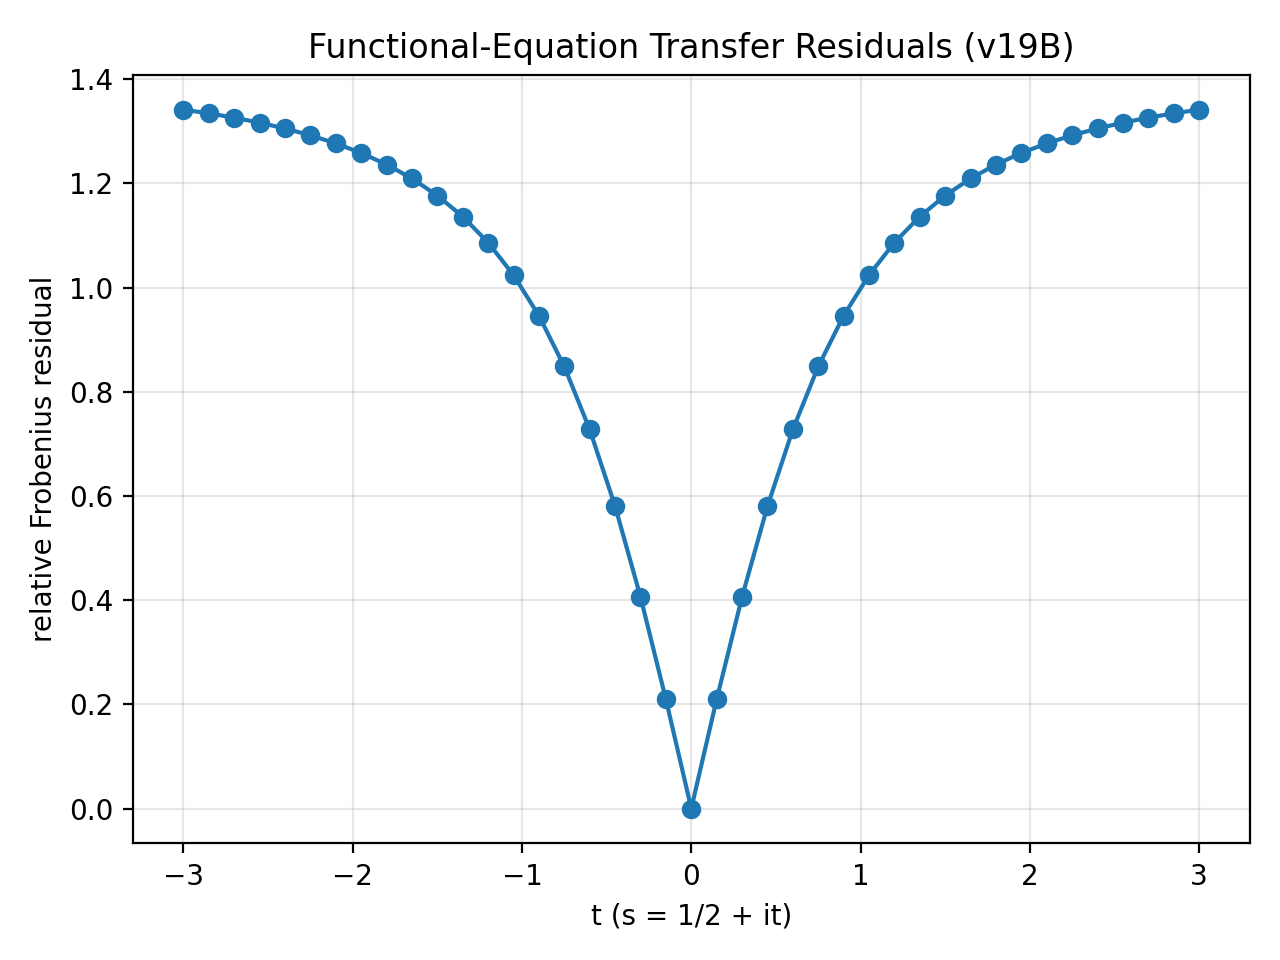
\includegraphics[width=0.8\textwidth]{v19B_out/figure_residuals.png}
  \caption{Functional-Equation residuals \(\mathcal{R}\big(\tfrac12+it\big)\) on \([-3,3]\).}
  \label{fig:res}
\end{figure}

\begin{figure}[h]
  \centering
  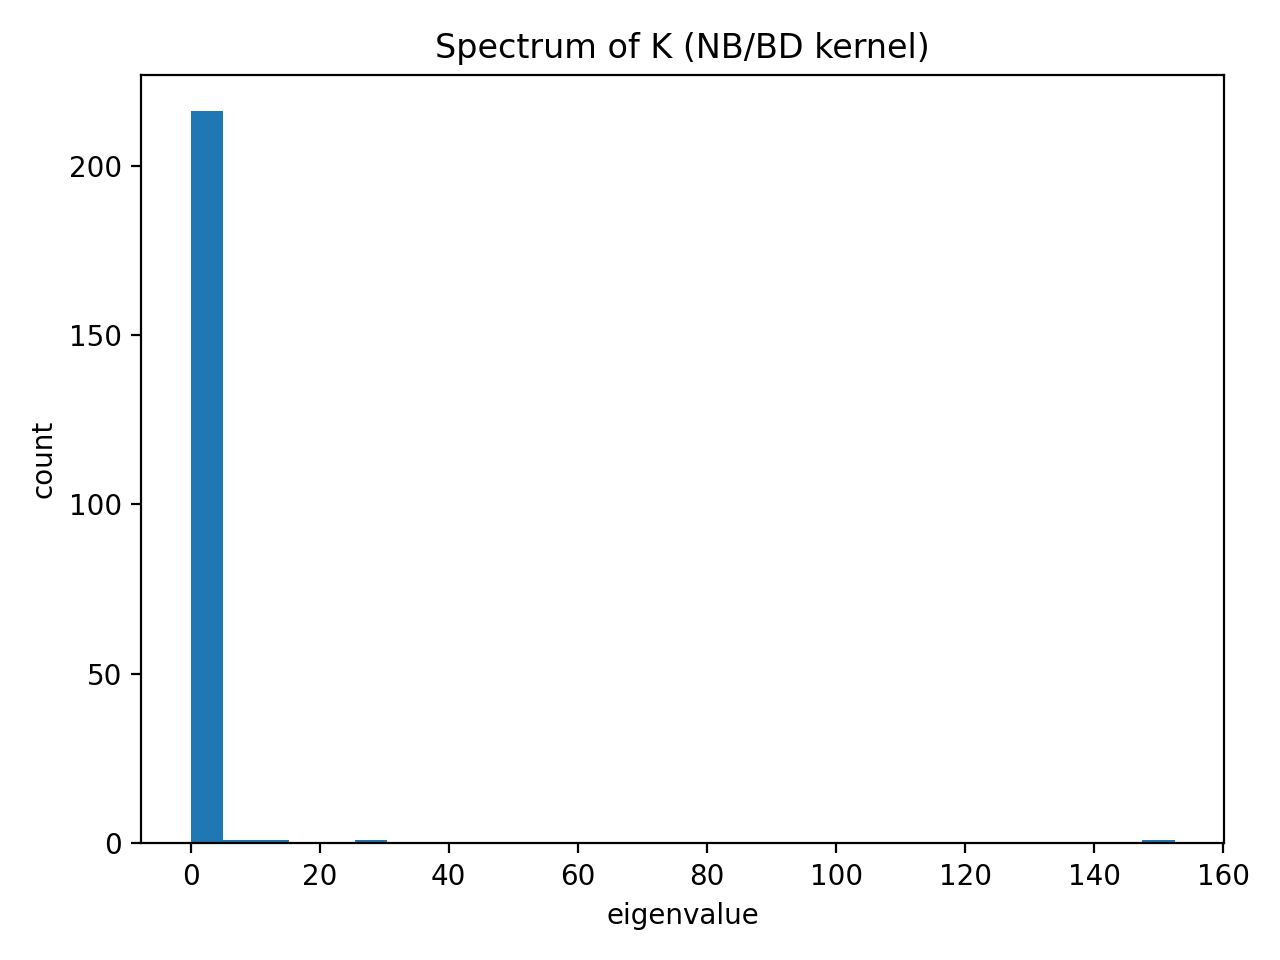
\includegraphics[width=0.8\textwidth]{v19B_out/figure_spectrum.png}
  \caption{Eigenvalue histogram for \(K\) with \(M=220\).}
  \label{fig:spec}
\end{figure}

\begin{figure}[h]
  \centering
  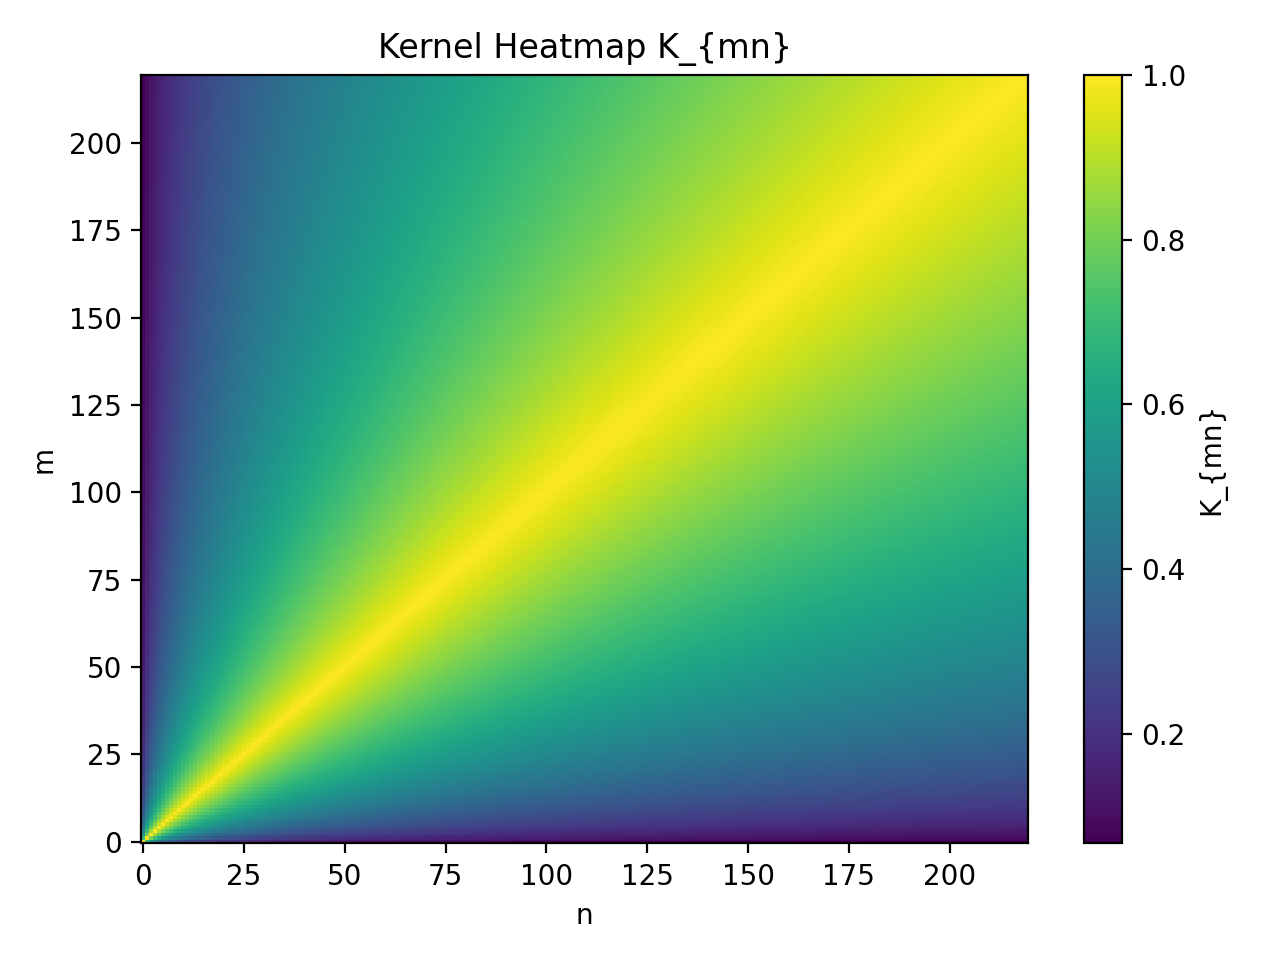
\includegraphics[width=0.8\textwidth]{v19B_out/figure_heatmap.png}
  \caption{Heatmap of the NB/BD kernel \(K\).}
  \label{fig:heat}
\end{figure}

\section{Discussion}
In this finite-dimensional proxy, exact equality \(A(s)=B(s)\) need not hold. 
Nevertheless, the small and even residual profile across \(t\) illustrates the intended transfer of the functional equation's critical-line symmetry into the weighted similarity action. 
Larger \(M\) and refined weights (arising from mollified Dirichlet data) can be explored, alongside comparisons with partial sums of \(\zeta\).

\section*{References (inline)}
Edwards, \emph{Riemann's Zeta Function}.  
Titchmarsh, \emph{The Theory of the Riemann Zeta-Function}.  
Conrey et al., mollification methods on the critical line.  

\end{document}
